\documentclass{article}

\usepackage[paper=letterpaper,margin=2.5cm]{geometry} % Set Margins

%% Math and math fonts
\usepackage{amsmath, amsthm, amssymb, amsfonts}
\usepackage{bbm} % for \mathbbm{1}

% date
\usepackage[nodayofweek]{datetime}

% Color
\usepackage{color, xcolor}

% Misc
\usepackage{environ}  % \collect@body in asmmath
\usepackage{graphicx} % \includegraphics options
\usepackage{mdframed} % text boxes
\usepackage{indentfirst} % Indent first paragraph after section header
\usepackage[shortlabels]{enumitem} % Control enumerate items with [(a)]
\usepackage{comment} % Comments
\usepackage{fancyhdr} % Headers and footers

% Tables
\usepackage{array}

% Sub-figures and figure placement
\usepackage{caption}
\usepackage{subcaption}
\usepackage{float} 

% Graphing
\usepackage{pgfplots}
\pgfplotsset{compat=1.17}
\usepackage{tikz}

% Title Placement
\usepackage{titling}
\setlength{\droptitle}{-6em}

%set indent to 
\setlength{\parindent}{0pt}

% Hyper refs
\usepackage{hyperref}
\hypersetup{
    colorlinks=true,
    linkcolor=blue,
    urlcolor  = blue,
    filecolor=magenta,      
    urlcolor=blue,
    citecolor = blue,
    anchorcolor = blue
}

% % Citation management
\usepackage{natbib}
\bibliographystyle{abbrvnat}
\setcitestyle{authordate,open={(},close={)}}

\pagestyle{fancy}

\usepackage[paper=letterpaper,margin=2.5cm]{geometry} % Set Margins

%% Math and math fonts
\usepackage{amsmath, amsthm, amssymb, amsfonts}
\usepackage{bbm} % for \mathbbm{1}

% date
\usepackage[nodayofweek]{datetime}

% Color
\usepackage{color, xcolor}

% Misc
\usepackage{environ}  % \collect@body in asmmath
\usepackage{graphicx} % \includegraphics options
\usepackage{mdframed} % text boxes
\usepackage{indentfirst} % Indent first paragraph after section header
\usepackage{comment} % Comments
\usepackage{fancyhdr} % Headers and footers

% Tables
\usepackage{array}

% Sub-figures and figure placement
\usepackage{caption}
% \usepackage{subcaption}
\usepackage{float} 

% Graphing
\usepackage{pgfplots}
\pgfplotsset{compat=1.17}
\usepackage{tikz}

% Title Placement
\usepackage{titling}
\setlength{\droptitle}{-6em}

%set indent to 
\setlength{\parindent}{0pt}

% Hyper refs
\usepackage{hyperref}
\hypersetup{
    colorlinks=true,
    linkcolor=blue,
    urlcolor  = blue,
    filecolor=magenta,      
    urlcolor=blue,
    citecolor = blue,
    anchorcolor = blue
}

% % Citation management
\usepackage{natbib}
\bibliographystyle{abbrvnat}
\setcitestyle{authordate,open={(},close={)}}

\newcolumntype{M}{>{$}c<{$}} % Define a new column type for math mode


% ----------------------------------------
% TITLE
% ----------------------------------------

\pagestyle{fancy}

\lhead{Creel}
\chead{Review}
\rhead{AMES}

\title{AMES Midterm Review}
\author{Andie Creel}

\begin{document}
\maketitle

\section{Exponential functions}
What does an exponential function really mean? 
\begin{align}
    f(x) = e^x\\
    f'(x) = e^x
\end{align}
$f(x)$ is a function where the \textbf{slope} of the function increases \textbf{by the rate that f(x)} is increasing. That is what the derivative of $e^x$ is still $e^x$. 

\section{Percent Change}
Let's say you have a function that models an outcome of interest, 
\begin{align}
    y = f(x)
\end{align}

Consider the case where you are interested in the percent change of that outcome (\textit{ie} \% change in $y$), rather than the level of the outcome (\textit{ie} $y$ itself). \\

What is a transformation of the function that would give us percent change in y? Taking of the derivative of the log of the function. 
\begin{align}
    g(x) &= ln(f(x))\\
    \text{\% change in y} &= g'(x)\\
    &= \frac{d ln(f(x))}{dx}\\
    &= \frac{1}{f(x)} f'(x) \\
    & = \frac{f'(x)}{f(x)}\\
    &= \frac{\Delta f(x)}{f(x)}
\end{align}
where we've used the properties of logs and the change rule. 
\begin{figure}[htp]
    \centering
        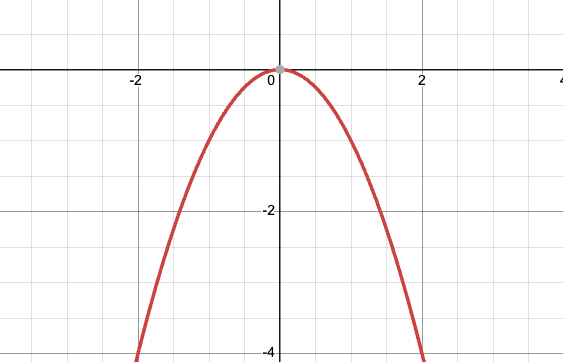
\includegraphics[width=0.35\textwidth]{Screen Shot 2023-10-23 at 4.53.45 PM.png}
    \caption{$-x^2$}
    % \label{fig:sample}
\end{figure}

\section{Draw graphs when you know what they are}
If you think you can draw a graph with the information you have, sketch it out. This will give you intuition. \\

Let's say I have the function $f(x) = -x^2$\\ 

What's the sign of the derivative when x is less than 0? (positive) \\

What's the sign of the derivative when x if greater than zero? (negative) \\

What's the sign if the derivative when $x = 0$? (zero)\\

All these questions are not-tedious to answer when looking at a graph, but harder without. 

\section{Finding max and min with first and second derivative}

Consider the function $f(x)$. \\

What level of $x$ maximizes or minimizes $f(x)$? We want to know when the slope is zero (at the top of the "mound"). Therefore to find the max or min, take the first derivative and set it equal to zero. Solve that equation for $x$, which will be the level of $x$ that maximizes $f(x)$. \\

How do we know if it's a max or min? Take the second derivative and plug in that value of x. If it's negative, then it's a maximum (frowny face). If it's positive, then it's a minimum (smiley face). 

\section{Taylor Series}

We know that straight lines are good approximates because a line is a conditional mean, and means are good at minimizing error.\\

Series are good approximators of sequences of numbers, because series are functions. \\

A \textbf{Taylor Series} is an extremely useful series for approximating the relationship of sequence of numbers (data is a sequence of numbers). Taylor series underpins a lot of the math we do today, particularly for any relationship that isn't linear. 

\begin{align}
    f(x) = f(a) + \frac{f'(a)}{1!}(x-a)^1 + \frac{f''(a)}{2!}(x-a)^2 + \frac{f'''(a)}{3!}(x-a)^3 + ... + \frac{f^k(a)}{k!}(x-a)^k + R
\end{align}
where $R$ is the residual.\\


\subsection{0th order Taylor Series}
Consider a 0th order taylor series: it would be a mean aka just a flat line equal to $f(a)$. \\

If you're only looking at the means of a dataset, that means you're doing a 0th order taylor approximation.

\subsection{First order Taylor Series}

Consider a first order taylor series: 
\begin{align}
    f(x) &= f(a) + \frac{f'(a)}{1!}(x-a)^1 \\
    &= A + B (x-a) \\
    &= A -aB + Bx\\
    &= m + Bx
\end{align}
It's a line with a slope. A first order Taylor series is a linear approximation. Linear regression is a first order Taylor approximation. \\

\subsection{Discussion of models}
Any Taylor Series approximation is a model. If someone says "I don't do models, let's only do means" they actually \textit{are} suggesting a model. A mean is a model, it's a zero order Taylor Series approximation! 

Higher order Taylor Series will approximate an underlying function better than a lower order. \textit{However,} we do not always have enough data to fit a higher order Taylor series because it would require more estimating parameters and your data set may not have enough power (aka enough data) to do so. \\

More on Taylor series: \url{https://github.com/a5creel/AMES/blob/main/class_notes/5_weds/main.pdf}. 

\section{pset 1 Q 1}
Function: 
\begin{align}
    f(x) &= x^2 ln(x^2)\\
\end{align}
first derivative: 
\begin{align}
    f'(x) &= 2x ln(x^2) + x^2 \frac{1}{x^2}2x\\
    &= 2x ln(x^2) + 2x \\
\end{align}
second derivative
\begin{align}
    f''(x) &= 2ln(x^2) + 2x \frac{1}{x^2} 2x + 2\\
    &= 2ln(x^2) + 6
\end{align}

To find point of inflection, set second derivative to 0 and solve for x
\begin{align}
    2ln(x^2) + 6 = 0\\
    ln(x^2) = -3 \\
    x^2 = exp(-3) \\
    x = exp(-3)^{1/2}
\end{align}

I think there is a typo for the inflection point in the answer key. 

\section{integration by parts }
section 2.1 and 2.2 \url{https://github.com/a5creel/AMES/blob/main/class_notes/6_weds/main.pdf}

\end{document}